\section{Autotools demo}

%https://www.gnu.org/savannah-checkouts/gnu/automake/manual/automake.html

\begin{frame}
    \frametitle{Steps for creating a \textit{C} project managed by Autotools}

    \alert{Phase \Romannum{1}: Initial setup}

    \begin{enumerate}
        \item Create and configure main \texttt{Makefile.am}.
        \item Create and configure \texttt{Makefile.am} in every subdirectories.
        \item Use \texttt{autoscan} to generate the starting point of \texttt{configure.scan}.
        \item Modify \texttt{configure.scan} with project settings into \texttt{configure.ac}.
        \item Use \texttt{autoreconf} to generate \texttt{./configure}.
    \end{enumerate}
    
\end{frame}

\begin{frame}
    \frametitle{Steps for creating a \textit{C} project managed by Autotools}

    \alert{Phase \Romannum{2}: Build}

    \begin{enumerate}
        \item Execute \texttt{./configure} to generate Makefiles.
        \item Execute \texttt{make} in the root directory of the project to build. (include testing)
        \item Execute \texttt{make install} in the root directory of the project to install.
    \end{enumerate}

    \alert{Phase \Romannum{3}: Prepare for distribution}

    \begin{enumerate}
        \item Execute \texttt{make clean} to remove build results in project.
        \item Execute \texttt{make distclean} to remove everything generated with \texttt{./configure}.
        \item Compress the directory (\texttt{*.tar.gz}) for release.
    \end{enumerate}
\end{frame}

\subsection{Phase \Romannum{1}: Initial setup}

\begin{frame}
    \frametitle{\Romannum{1}: ./Makefile.am}

    \begin{figure}[H]
        \centering
        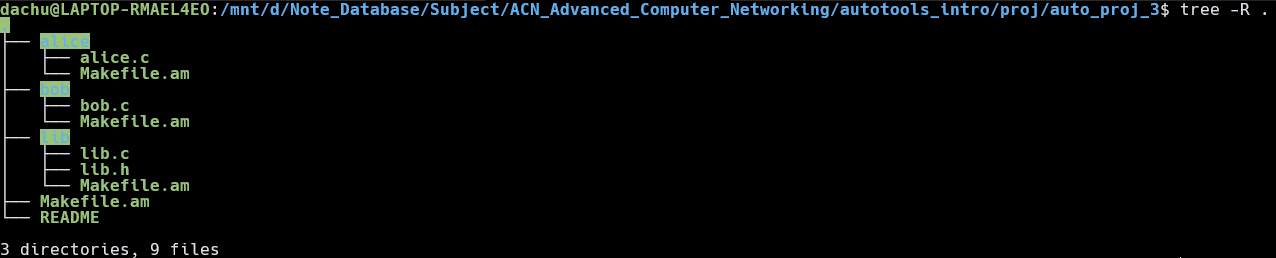
\includegraphics[width=0.9\textwidth]{../figure/autotool_init.png}
        \caption*{Tree structure after creating \texttt{Makefile.am}.}
    \end{figure}

    \begin{figure}[hp]
        \centering
        \hfill
        \begin{minipage}{.9\textwidth}
            \inputminted[
                mathescape,
                linenos,
                autogobble,
                fontsize=\scriptsize,
            ]{makefile}{E:\\GitHub\\presentation_in_LaTeX\\c_project_development\\proj\\auto_proj_3\\Makefile.am}
        \end{minipage}
        \hfill
        \caption*{Code for \texttt{./Makefile.am}.}
    \end{figure}
\end{frame}

\begin{frame}
    \frametitle{\Romannum{1}: Makefile.am for directory \texttt{alice} to build a binary}

    \begin{figure}[hp]
        \centering
        \hfill
        \begin{minipage}{.9\textwidth}
            \inputminted[
                mathescape,
                linenos,
                autogobble,
                fontsize=\tiny,
            ]{makefile}{E:\\GitHub\\presentation_in_LaTeX\\c_project_development\\proj\\auto_proj_3\\alice\\Makefile.am}
        \end{minipage}
        \hfill
        \caption*{Code for \texttt{./alice/Makefile.am}.}
    \end{figure}
\end{frame}

\begin{frame}
    \frametitle{\Romannum{1}: Makefile.am for directories \texttt{bob} to build a binary}

    \begin{figure}[hp]
        \centering
        \hfill
        \begin{minipage}{.9\textwidth}
            \inputminted[
                mathescape,
                linenos,
                autogobble,
                fontsize=\tiny,
            ]{makefile}{E:\\GitHub\\presentation_in_LaTeX\\c_project_development\\proj\\auto_proj_3\\bob\\Makefile.am}
        \end{minipage}
        \hfill
        \caption*{Code for \texttt{./bob/Makefile.am}.}
    \end{figure}
\end{frame}

\begin{frame}
    \frametitle{\Romannum{1}: Makefile.am for directory \texttt{lib} to build a LibTool library}

    \begin{figure}[hp]
        \centering
        \hfill
        \begin{minipage}{.9\textwidth}
            \inputminted[
                mathescape,
                linenos,
                autogobble,
                fontsize=\tiny,
            ]{makefile}{E:\\GitHub\\presentation_in_LaTeX\\c_project_development\\proj\\auto_proj_3\\lib\\Makefile.am}
        \end{minipage}
        \hfill
        \caption*{Code for \texttt{./lib/Makefile.am}.}
    \end{figure}
\end{frame}

\begin{frame}
    \frametitle{\Romannum{1}: \texttt{autoscan} for configure template \texttt{configure.scan}}

    \begin{figure}[hp]
        \centering
        \hfill
        \begin{minipage}{.9\textwidth}
            \inputminted[
                mathescape,
                linenos,
                autogobble,
                fontsize=\tiny,
            ]{bash}{E:\\GitHub\\presentation_in_LaTeX\\c_project_development\\proj\\auto_proj_3\\configure.scan}
        \end{minipage}
        \hfill
        \caption*{Scan result of the project structure in \texttt{configure.scan}.}
    \end{figure}
\end{frame}

\begin{frame}
    \frametitle{\Romannum{1}: \texttt{autoscan} for configure template \texttt{configure.ac}}

    \begin{figure}[hp]
        \centering
        \hfill
        \begin{minipage}{.9\textwidth}
            \inputminted[
                mathescape,
                linenos,
                autogobble,
                fontsize=\tiny,
                firstline=1,
                lastline=23,
            ]{bash}{E:\\GitHub\\presentation_in_LaTeX\\c_project_development\\proj\\auto_proj_3\\configure.ac}
        \end{minipage}
        \hfill
        \caption*{Modified \texttt{configure.ac}. (part 1)}
    \end{figure}
\end{frame}

\begin{frame}
    \frametitle{\Romannum{1}: \texttt{autoscan} for configure template \texttt{configure.ac}}

    \begin{figure}[hp]
        \centering
        \hfill
        \begin{minipage}{.9\textwidth}
            \inputminted[
                mathescape,
                linenos,
                autogobble,
                fontsize=\tiny,
                firstline=25,
                lastline=53,
            ]{bash}{E:\\GitHub\\presentation_in_LaTeX\\c_project_development\\proj\\auto_proj_3\\configure.ac}
        \end{minipage}
        \hfill
        \caption*{Modified \texttt{configure.ac}. (part 2)}
    \end{figure}
\end{frame}

\begin{frame}
    \frametitle{\Romannum{1}: \texttt{autoreconf -iv}}

    \begin{figure}[H]
        \centering
        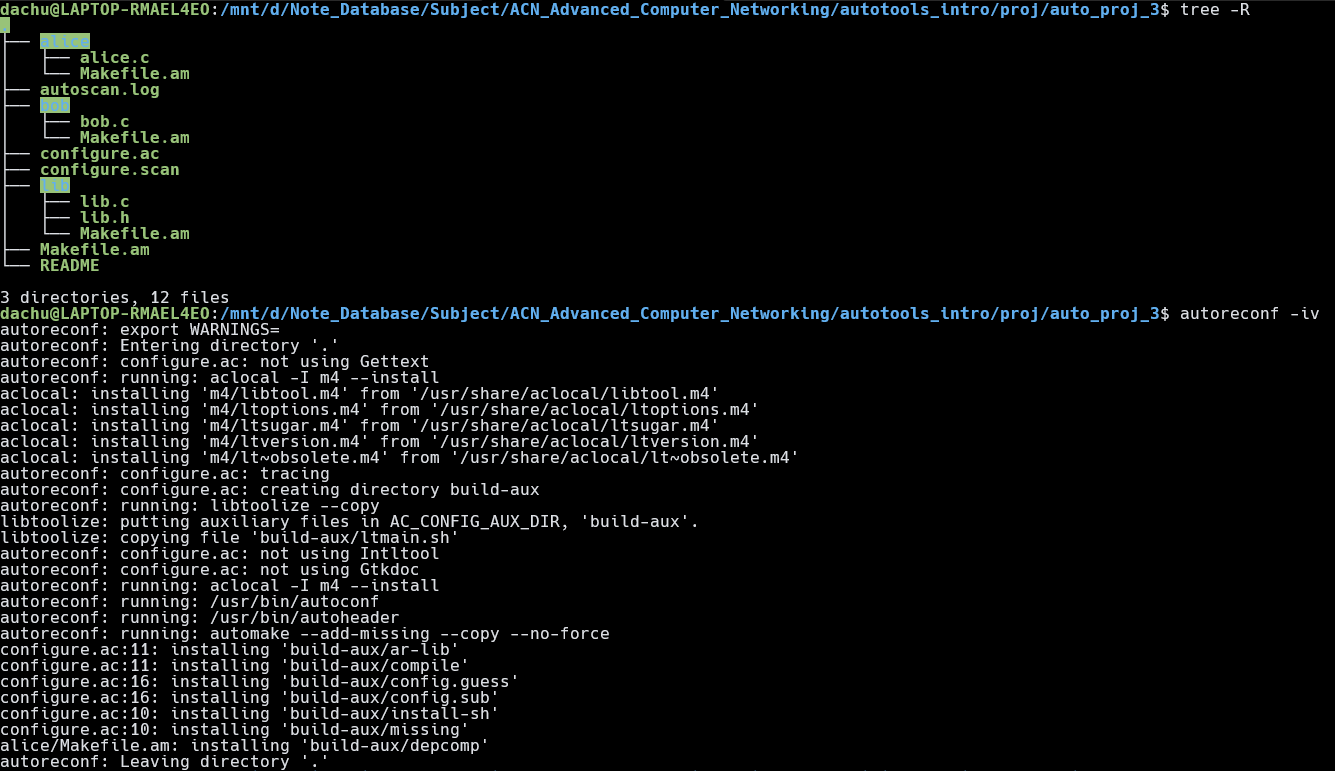
\includegraphics[width=0.9\textwidth]{../figure/autotool_1.png}
        \caption*{Generate auxiliary files.}
    \end{figure}
\end{frame}

\begin{frame}
    \frametitle{\Romannum{1}: \texttt{autoreconf -iv}}

    \begin{figure}[H]
        \centering
        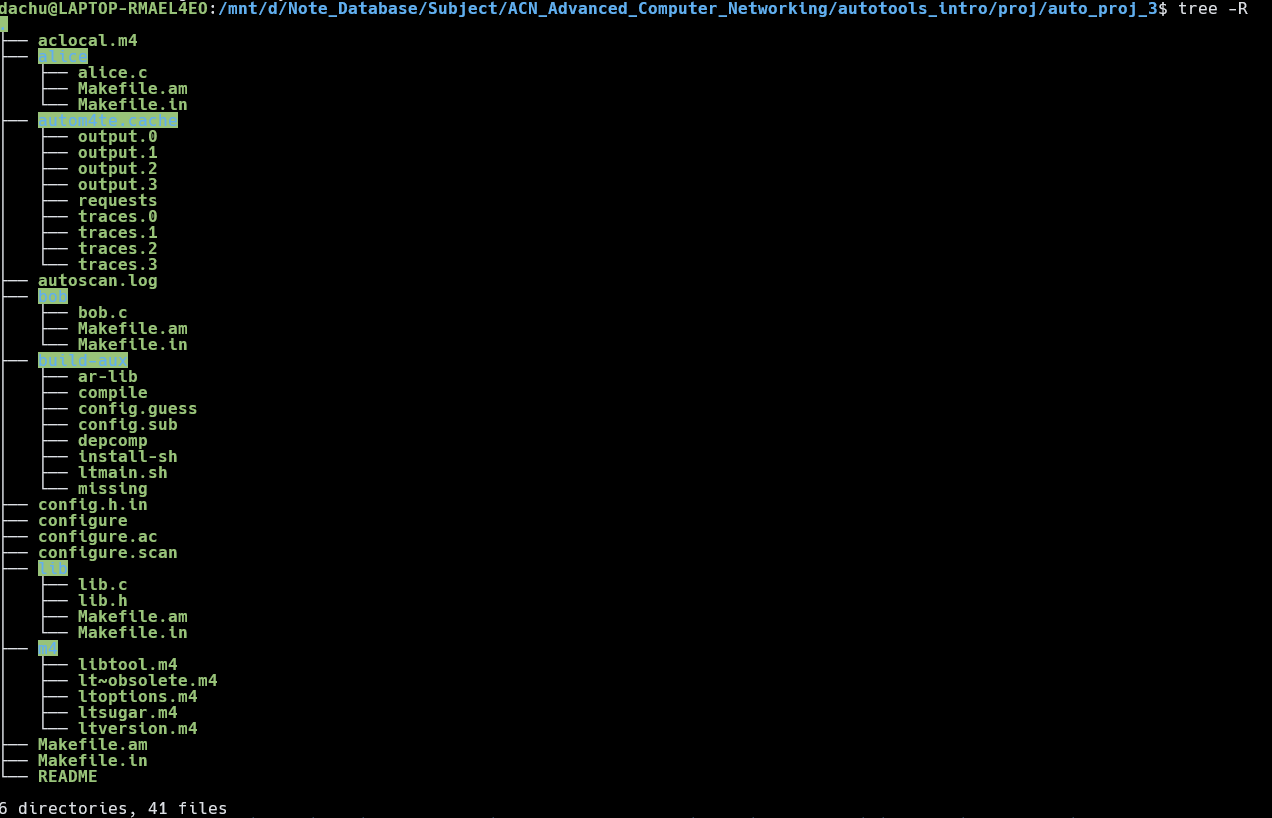
\includegraphics[width=0.9\textwidth]{../figure/autotool_2.png}
        \caption*{Tree structure of generate auxiliary files.}
    \end{figure}
\end{frame}

\subsection{Phase \Romannum{2}: Build}

\begin{frame}
    \frametitle{\Romannum{2}: \texttt{./configure}}

    \begin{figure}[H]
        \centering
        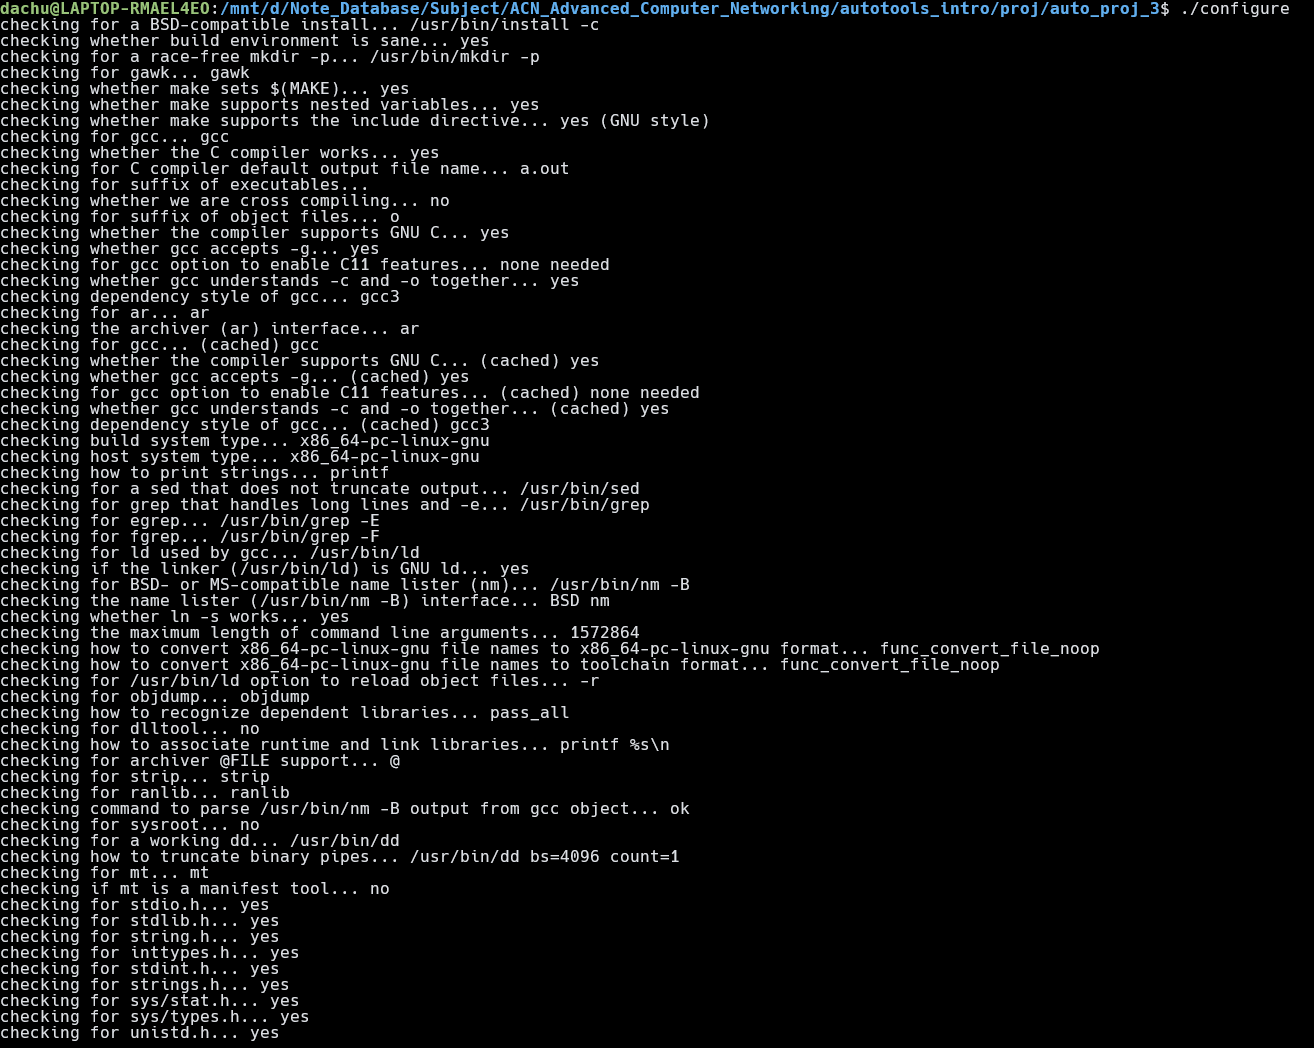
\includegraphics[width=0.7\textwidth]{../figure/autotool_3.png}
        \caption*{Generate Makefile for installing platform. (part 1)}
    \end{figure}
\end{frame}

\begin{frame}
    \frametitle{\Romannum{2}: \texttt{./configure}}

    \begin{figure}[H]
        \centering
        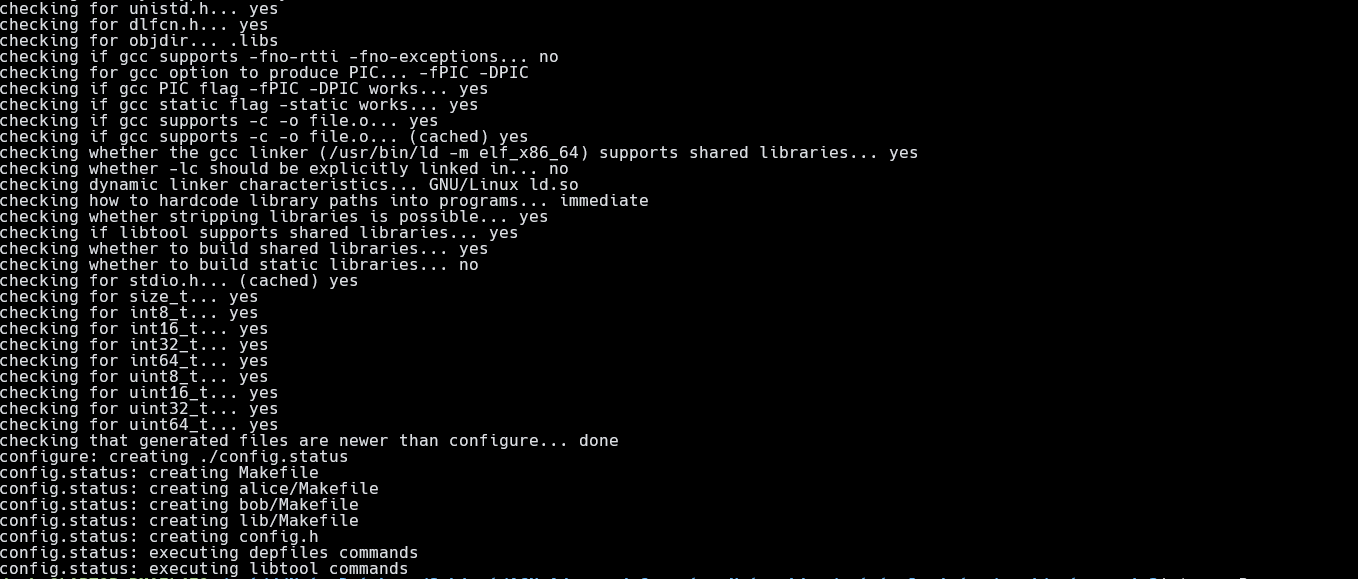
\includegraphics[width=0.8\textwidth]{../figure/autotool_4.png}
        \caption*{Generate Makefile for installing platform. (part 2)}
    \end{figure}
\end{frame}

\begin{frame}
    \frametitle{\Romannum{2}: \texttt{./configure}}

    \begin{figure}[H]
        \centering
        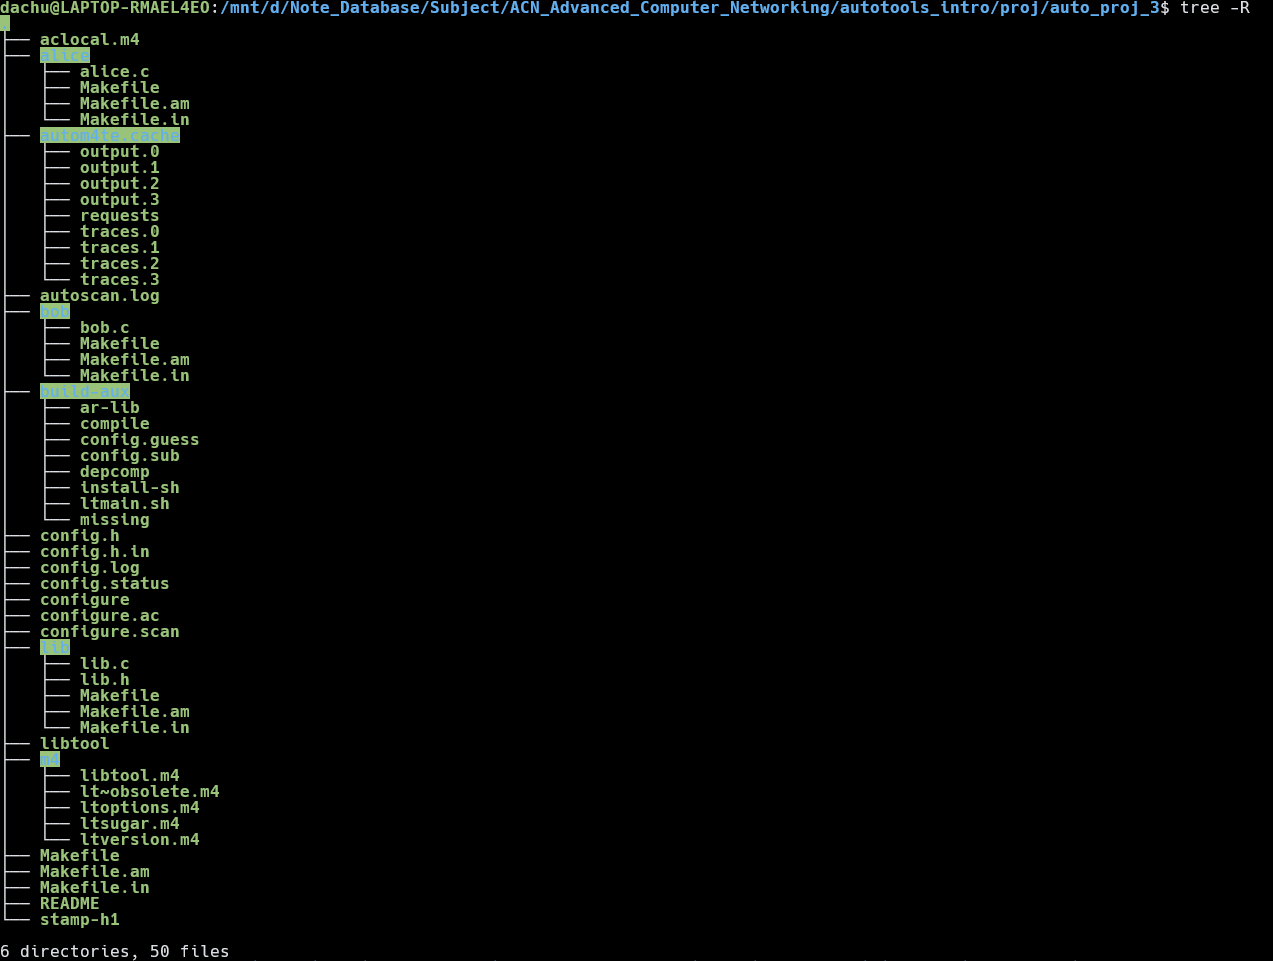
\includegraphics[width=0.7\textwidth]{../figure/autotool_5.png}
        \caption*{Tree structure of generated files including \texttt{Makefile}.}
    \end{figure}
\end{frame}

\begin{frame}
    \frametitle{\Romannum{2}: \texttt{make}}

    \begin{figure}[H]
        \centering
        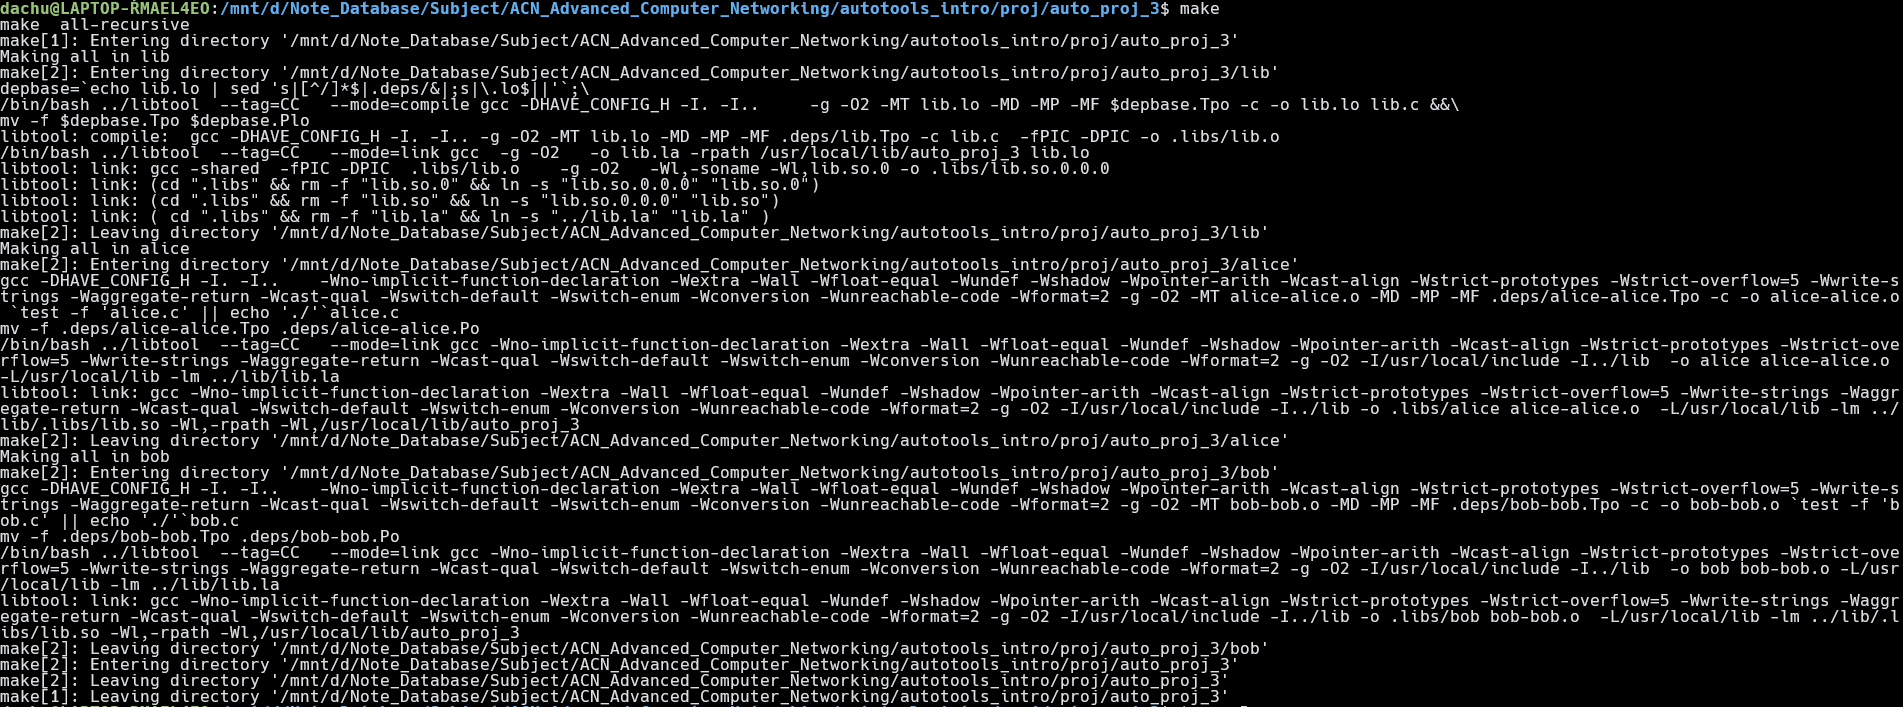
\includegraphics[width=0.95\textwidth]{../figure/autotool_6.png}
        \caption*{Project building.}
    \end{figure}
\end{frame}

\begin{frame}
    \frametitle{\Romannum{2}: \texttt{make}}

    \begin{figure}[H]
        \centering
        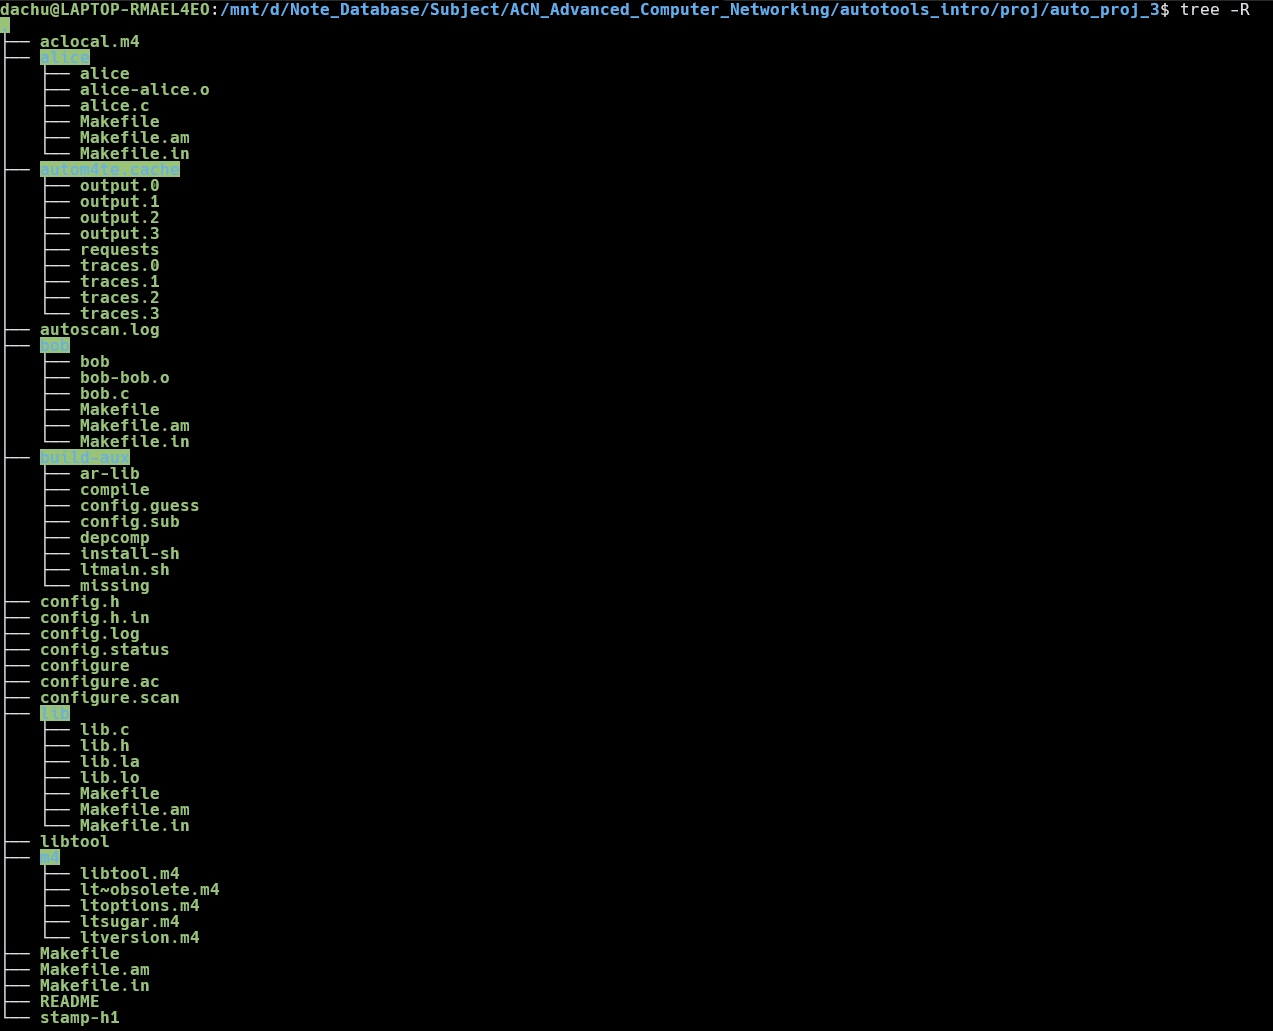
\includegraphics[width=0.7\textwidth]{../figure/autotool_7.png}
        \caption*{Tree structure of built project.}
    \end{figure}
\end{frame}

\begin{frame}
    \frametitle{\Romannum{2}: \texttt{make install}}

    \begin{figure}[H]
        \centering
        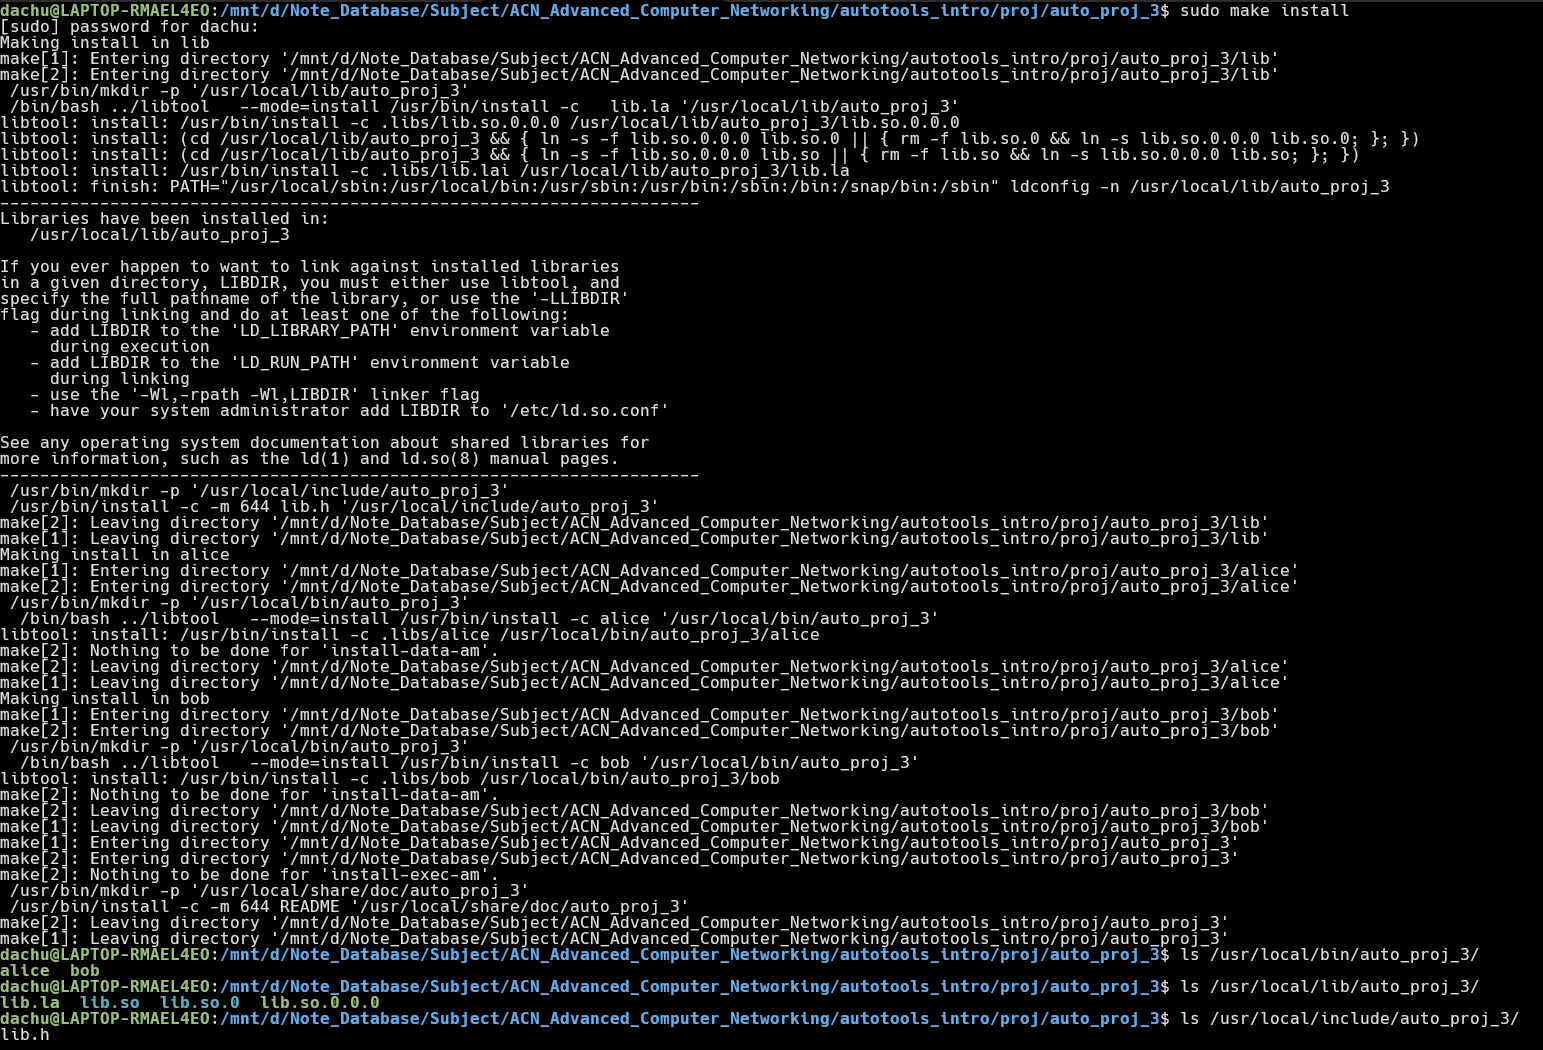
\includegraphics[width=0.8\textwidth]{../figure/autotool_8.png}
        \caption*{Execution result and installed files.}
    \end{figure}
\end{frame}

\begin{frame}
    \frametitle{\Romannum{2}: \texttt{make uninstall}}

    \begin{figure}[H]
        \centering
        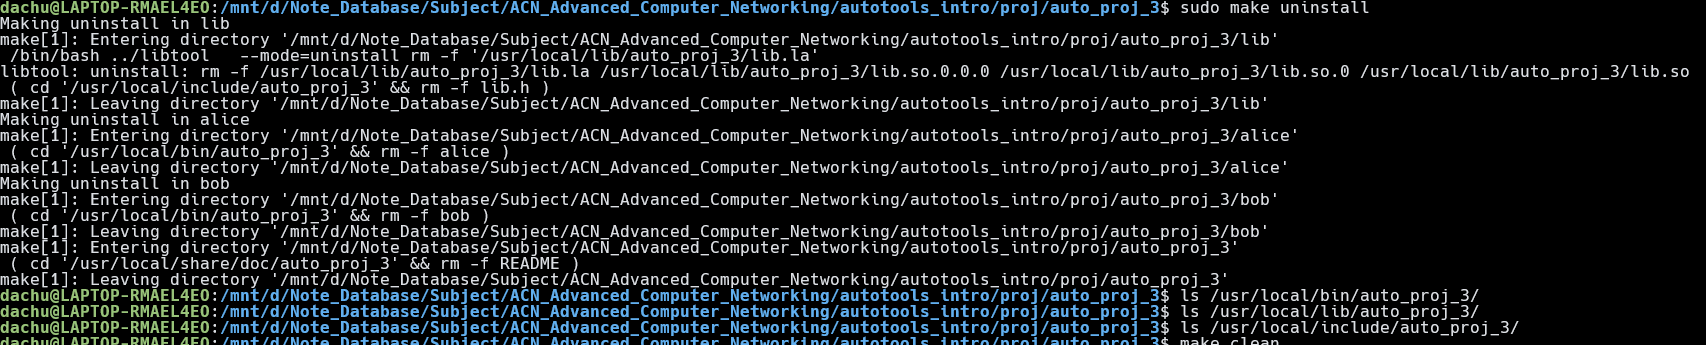
\includegraphics[width=0.9\textwidth]{../figure/autotool_9.png}
        \caption*{Removing all installed files.}
    \end{figure}
\end{frame}

\subsection{Phase \Romannum{3}: Prepare for distribution}

\begin{frame}
    \frametitle{\Romannum{3}: \texttt{make clean}}

    \begin{figure}[H]
        \centering
        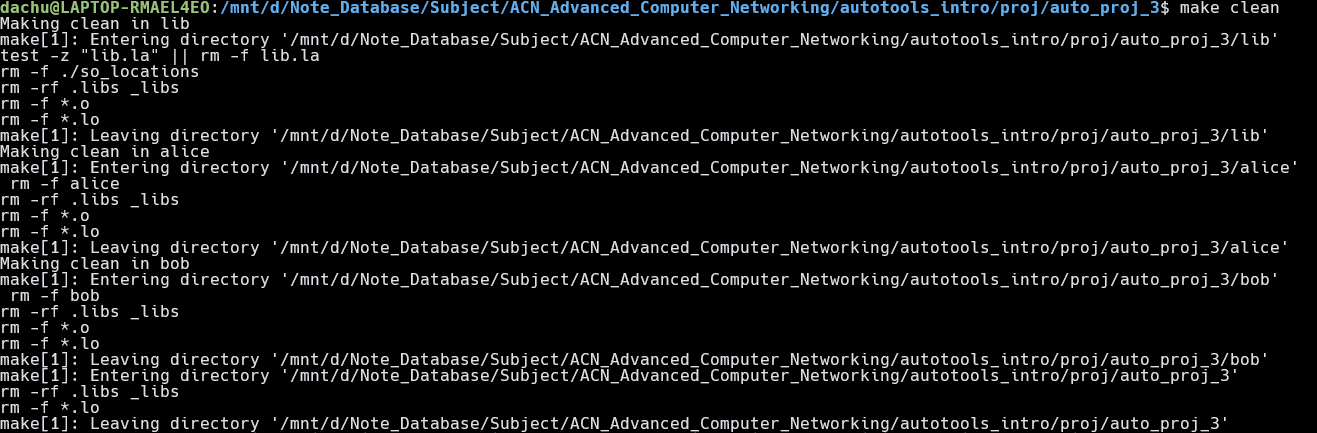
\includegraphics[width=0.9\textwidth]{../figure/autotool_10.png}
        \caption*{Remove all compiled files.}
    \end{figure}
\end{frame}

\begin{frame}
    \frametitle{\Romannum{3}: \texttt{make clean}}

    \begin{figure}[H]
        \centering
        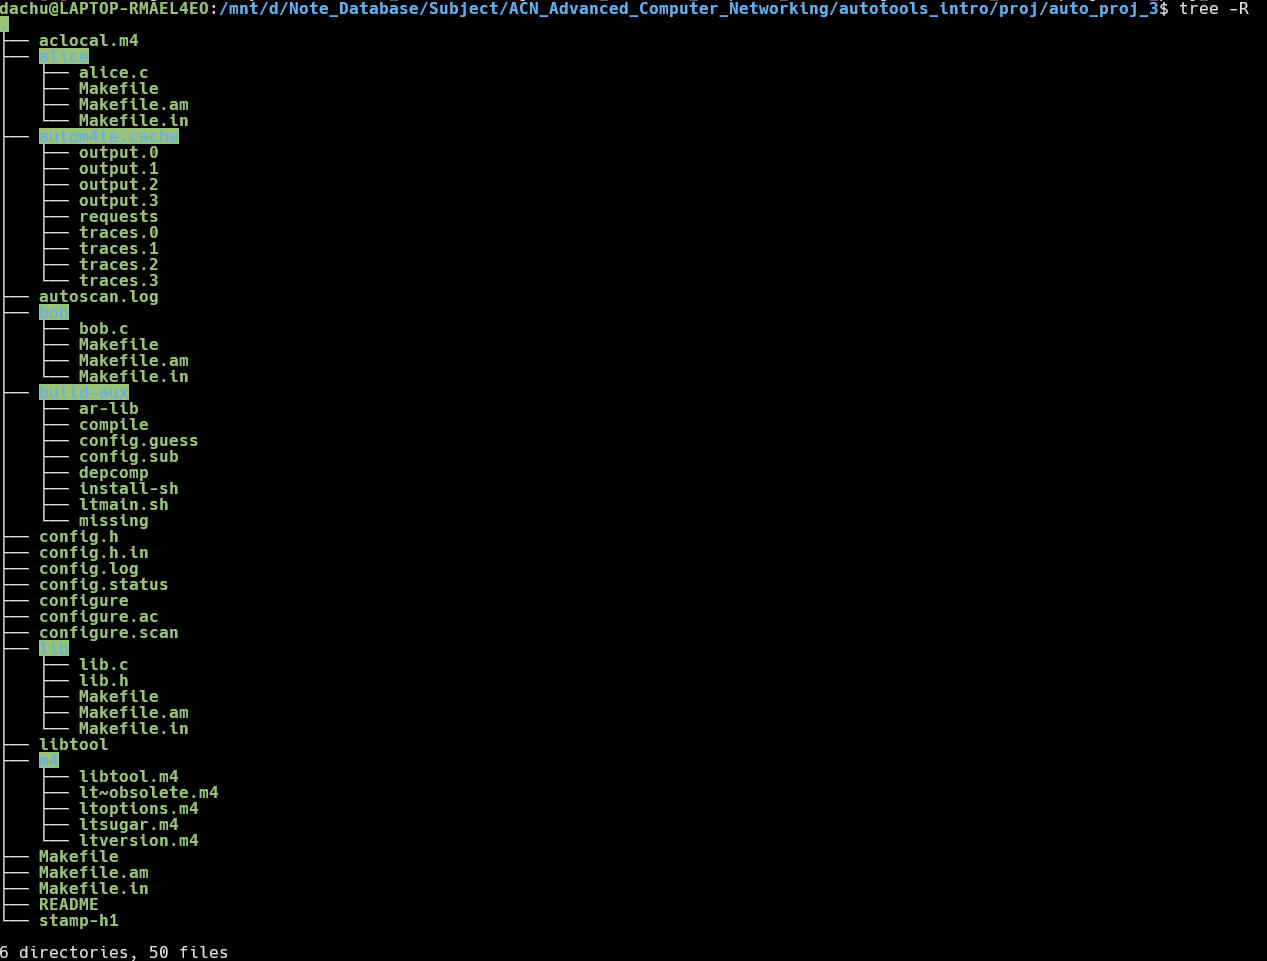
\includegraphics[width=0.7\textwidth]{../figure/autotool_11.png}
        \caption*{Tree structure after execution.}
    \end{figure}
\end{frame}

\begin{frame}
    \frametitle{\Romannum{3}: \texttt{make distclean}}

    \begin{figure}[H]
        \centering
        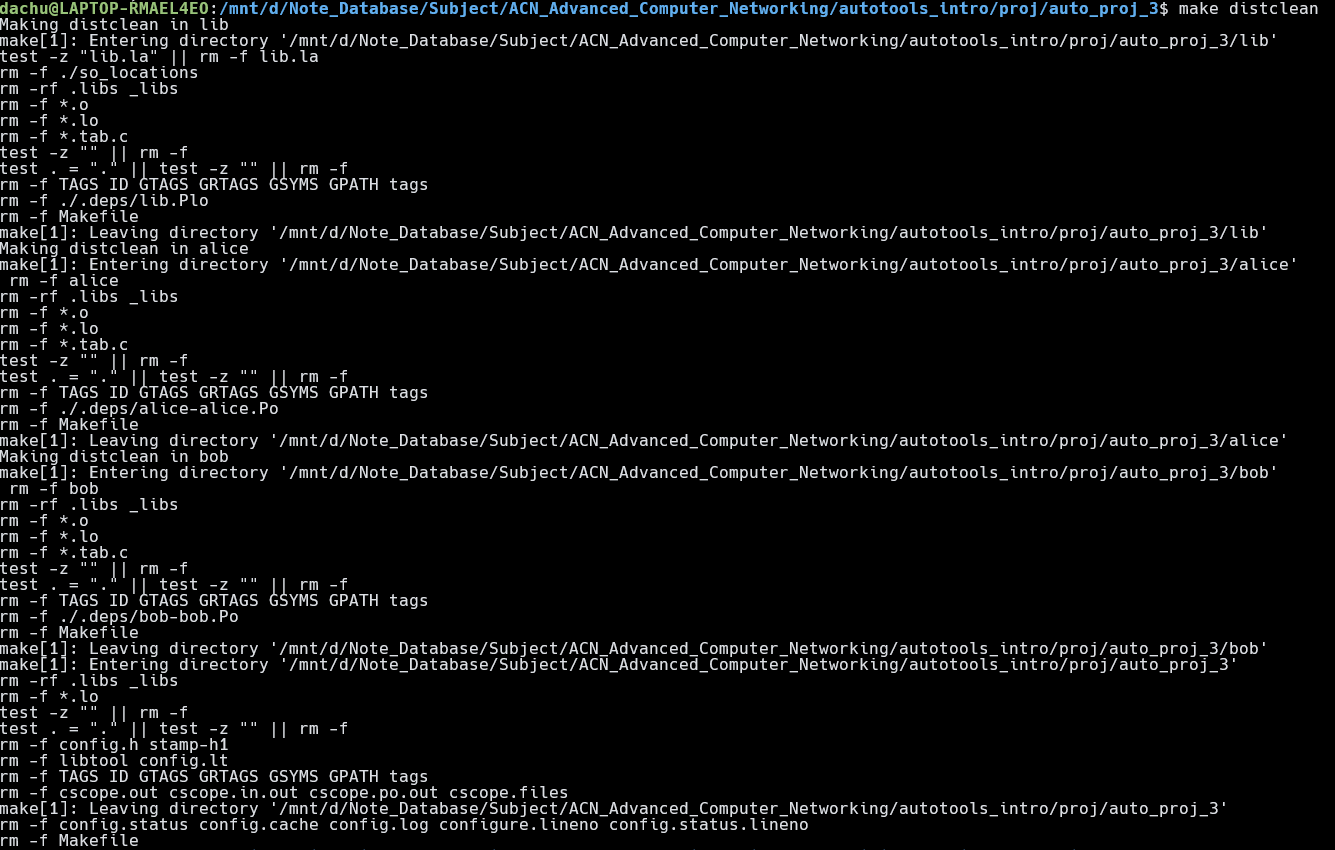
\includegraphics[width=0.8\textwidth]{../figure/autotool_12.png}
        \caption*{Remove almost all files generated from \texttt{./configure}.}
    \end{figure}
\end{frame}

\begin{frame}
    \frametitle{\Romannum{3}: \texttt{make distclean}}

    \begin{figure}[H]
        \centering
        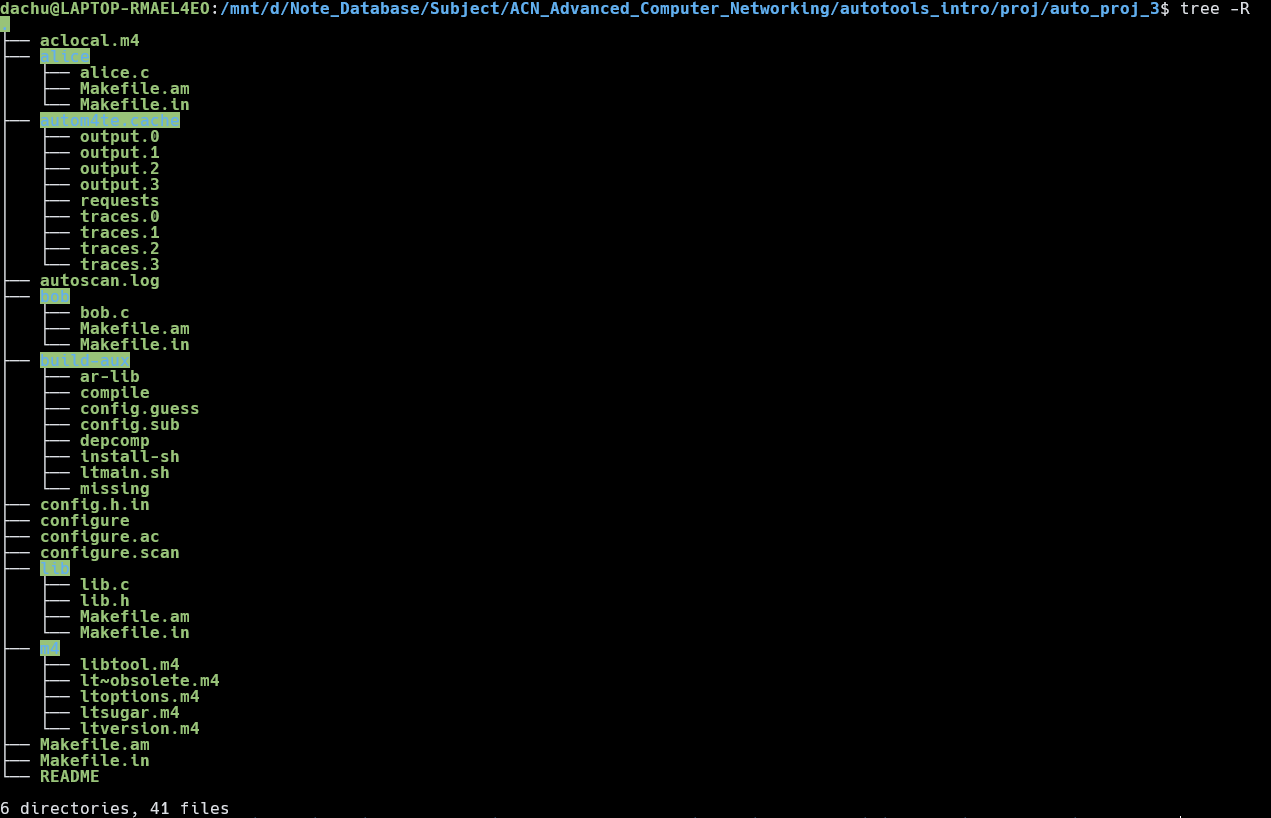
\includegraphics[width=0.8\textwidth]{../figure/autotool_13.png}
        \caption*{Tree structure after execution.}
    \end{figure}
\end{frame}
